\section{Dataset}
\label{sec:dataset}

We introduce a dataset for the SAVNav task, in which an embodied agent must navigate to an acoustic target while interpreting social sound events as spatial social boundaries. Unlike conventional audio-visual navigation, which treats sound primarily as a goal, and unlike vision-based social navigation, which reasons only about LOS humans, the SAVNav task requires the embodied agent to jointly reason about acoustic targets and spatial social boundaries.

\subsection{Task Definition and Scenarios}
\label{subsec:dataset-task}

The SAVNav task is situated in continuous indoor environments populated by static obstacles and dynamic human actors. The environment generates two classes of auditory signals: target sound events emitted by specific objects (e.g., doorbells, televisions) or humans (e.g., a human verbally calling the agent), and social sound events (e.g., footsteps, conversations) emitted continuously or intermittently by human actors.

The objective of the embodied agent is to navigate to the designated acoustic target using egocentric visual and auditory sensors, alongside real-time pose estimation and a pre-computed map of the static environment. Crucially, the agent must treat the social sound events as boundaries. The agent does not have access to the ground-truth locations or trajectories of the human actors and must infer their presence---even when fully occluded by walls or corners---proactively yielding to avoid collisions and personal space violations.

To evaluate the agent across different physical and social contexts, we structure the dataset into three scenarios, summarized in Table~\ref{tab:dataset_tiers} and with representative examples illustrated in Fig.~\ref{fig:dataset_sim}. The human counts specified below denote solely the distractor entities acting as social boundaries. When the acoustic target itself is a human, one additional stationary human actor is spawned to emit the target sound. This taxonomy separates LOS social routing from NLOS acoustic anticipation while still covering mixed domestic settings:

\begin{enumerate}
	\item \textit{Crowded Social:} A high-density, fully LOS environment containing two to four distractor humans (mean $3.2$). It comprises a single stationary conversational group (SCG)---a cluster of two to three humans gathered around a shared conversation centroid within a $1.25\,\mathrm{m}$ radius, each oriented toward the centroid and jointly emitting one \texttt{conversation} sound event---alongside up to one dynamic pedestrian (DP). The primary requirement is to navigate through socially dense spaces without interrupting ongoing conversations or violating personal space.
	\item \textit{Hidden Boundary:} A setting focused on anticipating NLOS social risks. The scene contains one to three distractor humans entirely occluded by geometry, functioning either as an approaching pedestrian (1 DP) or as a combination of a pedestrian and a two-person conversational group (1 SCG and 1 DP). This configuration tests the agent's ability to map acoustic cues to spatial layout and proactively yield at blind corners.
	\item \textit{Mixed Home Activity:} A complex domestic scenario with three to four distractor humans (mean $3.7$) that simultaneously presents LOS and NLOS social boundaries. It couples one NLOS dynamic pedestrian, whose trajectory is forced to intersect the agent's route as in the hidden boundary scenario, with one LOS stationary conversational group (two to three humans). This scenario evaluates whether the agent can jointly balance immediate visible social constraints with acoustically inferred NLOS risks.
\end{enumerate}

\begin{table}[t]
	\centering
	\caption{The SAVNav dataset comprises three scenarios: crowded social, hidden boundary, and mixed home activity. Social composition specifies distractor stationary conversational groups (SCGs) and dynamic pedestrians (DPs) across line-of-sight (LOS) and non-line-of-sight (NLOS) conditions, excluding the human acoustic target.}
	\label{tab:dataset_tiers}
	\resizebox{\linewidth}{!}{
		\begin{tabular}{lccl}
			\toprule
			Scenario            & Distractors & Visibility & Social Composition   \\
			\midrule
			Crowded Social      & 2--4        & LOS        & 1 SCG + 0--1 DP \\
			Hidden Boundary     & 1--3        & NLOS       & 0--1 SCG + 1 DP \\
			Mixed Home Activity & 3--4        & Mixed      & 1 SCG + 1 DP    \\
			\bottomrule
		\end{tabular}
	}
\end{table}

\begin{figure*}[t]
	\centering
	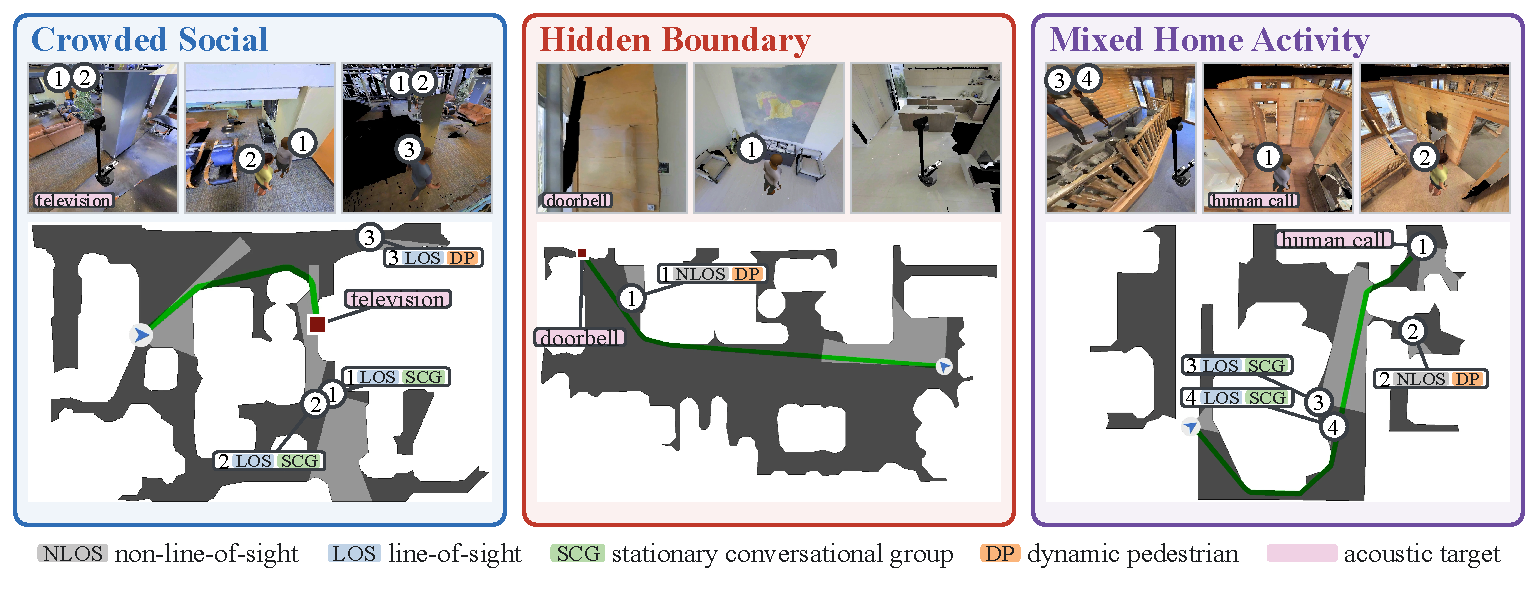
\includegraphics[width=\linewidth]{figures/scene.pdf}
	\caption{Representative episodes from the three scenarios in the SAVNav dataset. Each panel shows three third-person views (top) and the corresponding top-down map (bottom) with the ground-truth shortest path (green line) from the robot start pose (blue arrow) to the acoustic target. Numbered circles mark the human actors, with matching numbers overlaid on the views; callouts classify each human as line-of-sight (LOS) or non-line-of-sight (NLOS) and as part of a stationary conversational group (SCG) or a dynamic pedestrian (DP). Pink labels mark each episode's acoustic target.}
	\label{fig:dataset_sim}
\end{figure*}


\subsection{Simulation and Episode Generation}
\label{subsec:dataset-sim}

The dataset is built upon a high-fidelity simulator that integrates multi-agent human behaviors (Habitat 3.0~\cite{Habitat30Cohabitat2023}) with physically grounded acoustic rendering (SoundSpaces 2.0~\cite{SoundSpaces20Simulation2022}). To ensure diverse and realistic interactions, we utilize large-scale indoor environments from the Matterport3D dataset~\cite{Matterport3DLearningRGBD2017}. Within each episode, all task-relevant entities and acoustic sources are strictly confined to a single planar floor comprising no more than 10 rooms. The generated evaluation dataset comprises 1{,}008 episodes distributed evenly across the three scenarios (336 each) and the four acoustic target categories (252 each), sampled from 10 distinct scenes. Fig.~\ref{fig:dataset_stats} summarizes its social, spatial, and acoustic statistics.

\begin{figure}[t]
	\centering
	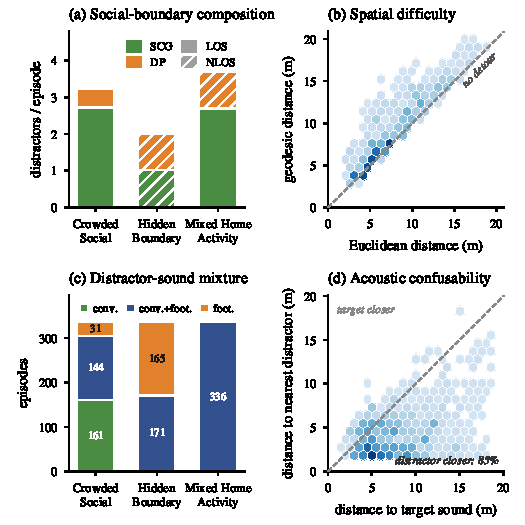
\includegraphics[width=\linewidth]{figures/dataset_stats.pdf}
	\caption{Statistics of the 1{,}008-episode SAVNav evaluation set. (a) Per-scenario social-boundary composition, decomposed into stationary conversational group (SCG) and dynamic pedestrian (DP) humans under line-of-sight (LOS) and non-line-of-sight (NLOS) visibility. (b) Spatial difficulty: geodesic versus Euclidean start--goal distance; points above the diagonal require detours around obstacles. (c) Distractor-sound mixture per scenario (\texttt{conversation} only, \texttt{conversation}+\texttt{footsteps}, or \texttt{footsteps} only). (d) Acoustic confusability: geodesic distance to the target sound versus to the nearest distractor sound; in $85\%$ of episodes a distractor is acoustically closer than the target, so the agent cannot simply home in on the loudest source.}
	\label{fig:dataset_stats}
\end{figure}

To ensure episodes accurately reflect the scenarios, we enforce strict parametric settings during generation.

\subsubsection{Acoustic Configurations}
To populate the simulated environment with realistic auditory cues, we curate a collection of 176 audio samples spanning the six defined sound event categories. Following the AudioSet Ontology~\cite{AudioSetOntology2017}, we organize these into target sound events (\texttt{doorbell}, \texttt{human call}, \texttt{television}, \texttt{water tap}) and social sound events (\texttt{conversation}, \texttt{footsteps}). These samples are sourced from BeDAViN~\cite{AudiovisualNavigationNoisy2025}, FSD50K~\cite{FSD50KOpenDataset2022}, and Freesound\footnote{\url{https://freesound.org/}} under Creative Commons licenses.

During episode initialization, up to three active sound sources are spatially anchored according to their semantic roles. Most acoustic targets are attached to their corresponding static objects within the Matterport3D scene (e.g., a door for \texttt{doorbell} or a sink for \texttt{water tap}), except for the \texttt{human call} target, which is anchored to a stationary human actor. Distractor social sound events (\texttt{conversation}, \texttt{footsteps}) are exclusively tied to human actors. Notably, the emission origin for \texttt{footsteps} tracks the dynamic pedestrian's position, emitting sound exclusively while the human actor is in motion. All audio samples are played on a continuous loop.

For acoustic rendering, we compute the room impulse responses (RIRs) between the active sound locations and the agent's microphone array using SoundSpaces 2.0. By convolving the dry audio waveforms with their respective RIRs and linearly superimposing the results, the simulator generates a single, continuous 4-channel FOA audio stream. This ensures that the embodied agent ultimately receives a physically grounded acoustic mixture of all concurrent sources intertwined with realistic room reverberations.

\subsubsection{Spatial and Dynamic Settings}
For the crowded social scenario, humans are spawned within the main topological pathways to force spatial negotiation. For the hidden boundary scenario, we use raycast initialization from the agent's starting pose to ensure the humans are strictly outside the agent's LOS. Furthermore, for DPs, we generate navigation waypoints such that their trajectory explicitly intersects with the agent's shortest geodesic path to the target. To ensure timely spatial conflicts, these NLOS DPs only begin moving when the agent approaches within a $3.0\,\mathrm{m}$ radius. This forced-intersection design guarantees that the agent cannot succeed by simply ignoring the human; it must proactively yield or alter its path based on approaching footsteps.

\subsubsection{ENMuS-Compatible Subset}
The released ENMuS\textsuperscript{3}~\cite{AudiovisualNavigationNoisy2025} weights are trained on a fixed BeDAViN target vocabulary, so a fair evaluation requires targets drawn from that in-distribution vocabulary. We therefore derive a $504$-episode subset (\texttt{water tap} and \texttt{television} targets only, $168$ episodes per scenario) by slicing the full evaluation set---without regeneration---and replacing each target recording with the corresponding ENMuS\textsuperscript{3} test-set sound (sink and TV monitor). The social boundaries, scenes, and episode geometry are otherwise identical to the full set. Because this subset is smaller and covers only two target categories, ENMuS\textsuperscript{3} results are reported separately and are not directly comparable to methods evaluated on the full $1{,}008$-episode set.

% \begin{figure*}[t]
% 	\centering
% 	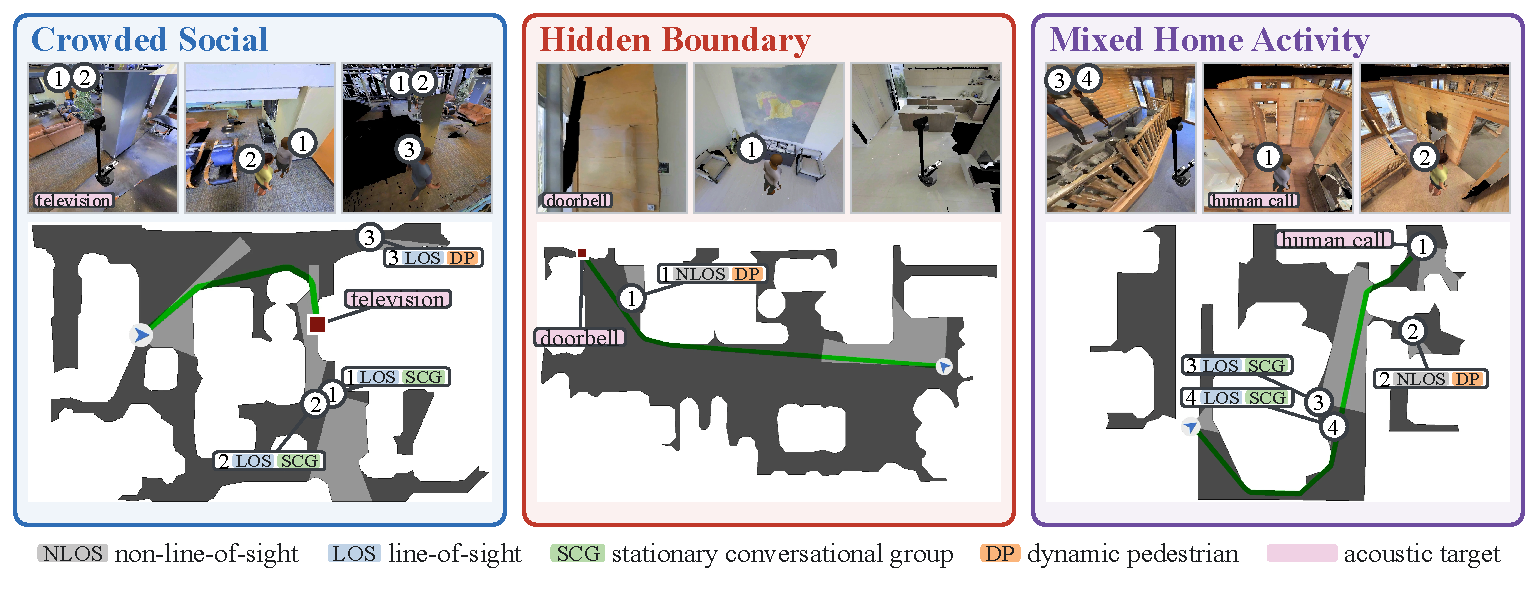
\includegraphics[width=\linewidth]{figures/scene.pdf}
% 	\caption{Representative episodes from the three scenarios in the SAVNav dataset. Each panel displays the third-person 3D views (top) and the corresponding top-down map (bottom) illustrating the ground-truth shortest path to the target (green line). The environments feature varying combinations of line-of-sight (LOS) and non-line-of-sight (NLOS) distractor humans, categorized as either stationary conversational groups (SCGs) or dynamic pedestrians (DPs).}
% 	\label{fig:dataset_sim}
% \end{figure*}

\subsection{Evaluation Metrics}
\label{subsec:dataset-metrics}

We evaluate the navigation system across three dimensions: task completion, human safety, and social compliance. Notably, reaching the target does not inherently imply safety, necessitating distinct social metrics.

\begin{enumerate}
	\item \textit{Success Rate (SR):} An episode is counted as a success if the agent executes the \texttt{stop} action within 500 time steps and its final distance to the acoustic target is $1.0\,\mathrm{m}$ or less without colliding with any human actor. Human collisions result in immediate episode failure.
	\item \textit{Success weighted by Path Length (SPL):} Measures navigation efficiency relative to the shortest traversable path and penalizes unnecessary detours.
	\item \textit{Success weighted by Time Length (STL):} A temporal analogue of SPL that measures execution efficiency in control steps rather than metric path length. We define $\mathrm{STL} = \frac{1}{N}\sum_{i=1}^{N} S_i \cdot \frac{T_i^*}{\max(T_i^*, T_i)}$, where $S_i$ is the binary success indicator, $T_i$ the number of control steps the agent takes, and $T_i^*$ the minimum number of steps required to traverse the shortest path at the nominal translational speed. It penalizes slow or hesitant execution that SPL, being purely geometric, cannot capture.
	\item \textit{Progress:} The fraction of the initial geodesic distance to the target that the agent closes, $\mathrm{Progress} = \mathrm{clip}\!\left((d_0 - d_f)/d_0,\, 0,\, 1\right)$, where $d_0$ and $d_f$ are the geodesic distances from the agent to the target at the start and end of the episode. Unlike SR, it credits partial approach on unsuccessful episodes and thus separates near-misses from complete failures.
	\item \textit{Human Collision Rate (HCR):} The fraction of episodes in which the agent collides with a human actor.
	\item \textit{NLOS Collision Rate (NCR):} The fraction of episodes terminating in a collision with a human who has been within the agent's camera field of view for less than $1.0\,\mathrm{s}$ prior to the impact. It quantifies the system's ability to avoid abrupt dynamic obstacles emerging from NLOS regions.
	\item \textit{Personal Space Compliance (PSC):} A measure of adherence to human social comfort zones. Following Falcon~\cite{CognitionPrecognitionFutureaware2025}, the social distance threshold is uniformly set to $1.0\,\mathrm{m}$ for all humans (dynamic or static), and the metric captures the fraction of time the agent maintains at least this distance relative to the episode length.
\end{enumerate}

% \subsection{Comparison with Existing Datasets}
% \label{subsec:dataset-compare}

% Table~\ref{tab:dataset_comparison} positions the SAVNav task against representative embodied navigation tasks. Standard audio-visual navigation evaluates acoustic target finding but does not model the social semantics of sound events. Vision-based social navigation evaluates behavior around humans but assumes LOS visibility. Emergency detection datasets such as HomeEmergency support audio-based exploration but do not include explicit social compliance with active human dynamics. The SAVNav task combines these requirements by asking the agent to use audio to anticipate and respect human activities even when they are fully occluded.

% \begin{table*}[t]
% 	\centering
% 	\caption{Comparison of the SAVNav task with representative embodied navigation tasks. The SAVNav task requires acoustic targets together with NLOS social compliance.}
% 	\label{tab:dataset_comparison}
% 	\begin{tabular}{lcccccc}
% 		\toprule
% 		Task                                                  & Goal Modality         & Human Dynamics & Social Compliance & Spatial Audio & NLOS Social Risk & Acoustic Target \\
% 		\midrule
% 		ObjectNav                                             & Vision                & No             & No                & No            & No               & No              \\
% 		SocialNav~\cite{CognitionPrecognitionFutureaware2025} & Vision                & Yes            & Yes               & No            & No               & No              \\
% 		AudioGoal~\cite{AudiovisualNavigationNoisy2025}       & Audio-Visual          & No             & No                & Yes           & No               & Partial         \\
% 		HomeEmergency~\cite{HomeEmergencyUsingAudio2025}      & Audio-Visual          & No             & No                & Yes           & No               & Yes             \\
% 		\textbf{SAVNav task (Ours)}                           & \textbf{Audio-Visual} & \textbf{Yes}   & \textbf{Yes}      & \textbf{Yes}  & \textbf{Yes}     & \textbf{Yes}    \\
% 		\bottomrule
% 	\end{tabular}
% \end{table*}
